\documentclass{article}

% Language setting
\usepackage[english]{babel}

% Set page size and margins
% Replace `letterpaper' with `a4paper' for UK/EU standard size
\usepackage[letterpaper,top=2cm,bottom=2cm,left=3cm,right=3cm,marginparwidth=1.75cm]{geometry}

% Useful packages
\usepackage{amsmath}
\usepackage{graphicx}
\usepackage[colorlinks=true, allcolors=blue]{hyperref}

\title{Deep learning lab - Assignment 1}
\author{Christian Altrichter}

\begin{document}
\maketitle


\section{Polynomial Regression [96/100 points]}

\subsection{Question 1.1}

The corresponding code snippet is provided in the code data file. The outcome of the the completion of the code in a range from -3 to 3 on the x axis is as follow:

\begin{figure}[!htb]
\centering
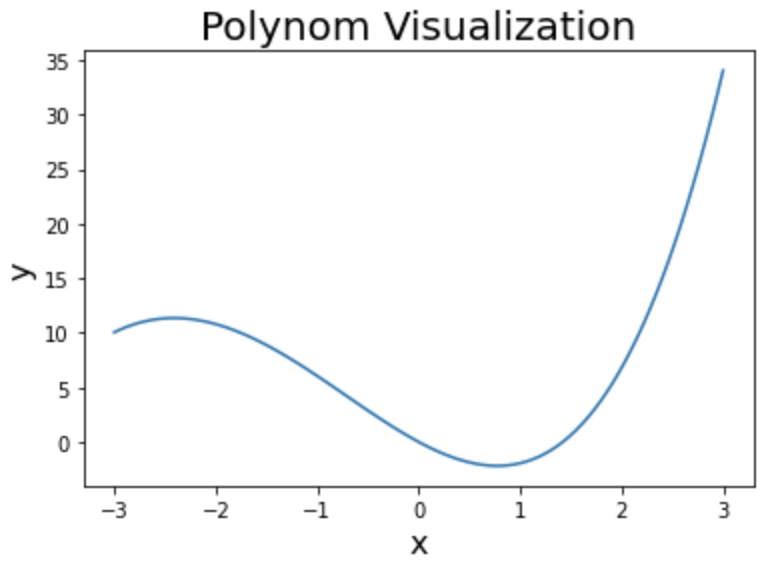
\includegraphics[scale = 0.8]{Question1_Graph.png}
\caption{\label{fig:fig}Graph for Question 1.1, plotting the given polynom}
\end{figure}

\subsection{Question 1.2}

The code has been completed and no special functions were required.

\subsection{Question 1.3}

Here, the two data sets were created with a seed of 0 and 1. the only special function used was the one completed in Question 1.2.

\subsection{Question 1.4}

In the following the two graphs are depicted based on the two data sets created from Question 1.4

\begin{figure}[!htb]
\centering
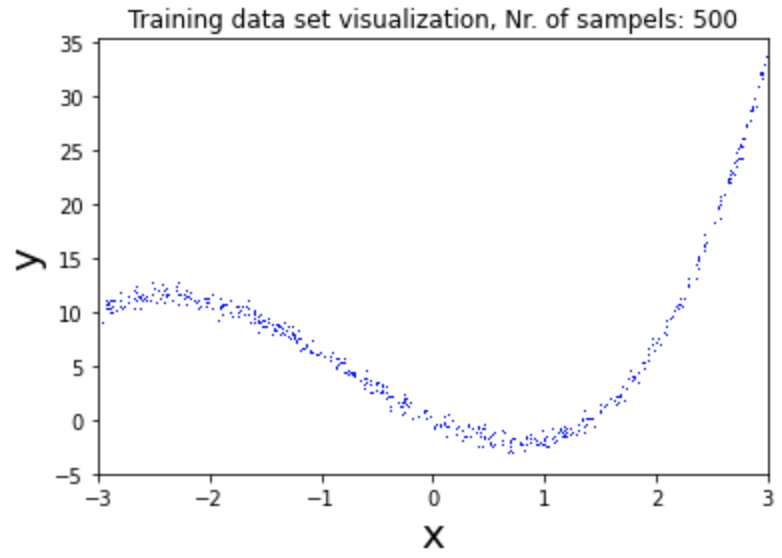
\includegraphics[scale = 0.8]{Question4_Graph1.png}
\caption{\label{fig:fig}Graph for Question 1.4, scatter plot of the test data}
\end{figure}

\begin{figure}[!htb]
\centering
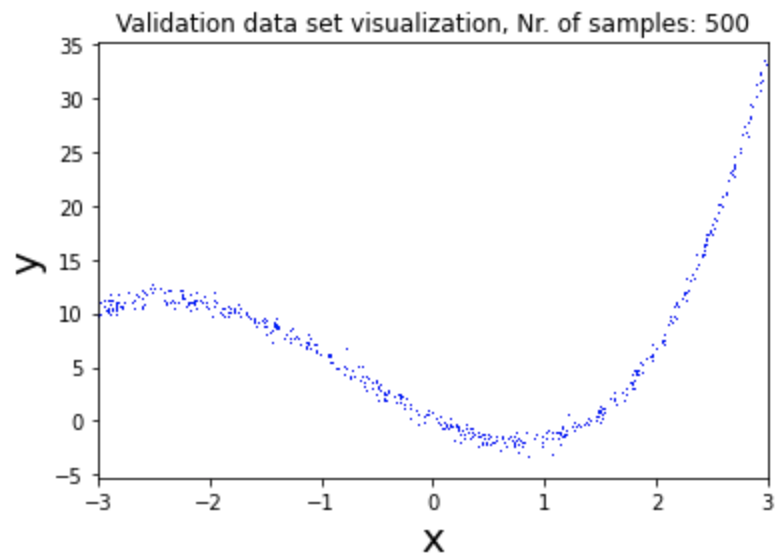
\includegraphics[scale = 0.8]{Question4_Graph2.png}
\caption{\label{fig:fig}Graph for Question 1.4, scatter plot of the validation data}
\end{figure}

\subsection{Question 1.5}

  If the bias is set to True, a randomly generated bias is added to the output where the bias is in dependency to the input. Here, bias is calculated by \[k = \frac{1}{'in_features'} \] and then randomized between \[[-\sqrt{k} \rightarrow \sqrt{k}] \]. However, if it is set to false, then the bias is set to 0. The function \[y = x*W^T + b\] where x is our input, W is the weight and b the bias. For example: 
  Bias is often used to adapt for over/under-fitting models. Should the model be under-fitted, we can increase the complexity of the model (e.g. extra features). Should the model be over-fitted, we can reduce the complexity by increasing the bias, e.g. reducing the number of features. 
  In our model we do not need it because we have a a validation set to which we can compare our results. \newline

  Sources used: 
  \begin{itemize}
  \item https://pytorch.org/docs/stable/generated/torch.nn.Linear.html
  \item https://www.youtube.com/watch?v=QpyXyenmtTA
  \item https://www.youtube.com/watch?v=djRh0Rkqygw
\end{itemize}
  
  \textbf{Convolutional sets and unsupvervised?
  Using equations? CHECK AGAIN!!!}


\subsection{Question 1.6}

The adapted code for Question 1.6 can be found in the source file.

\subsection{Question 1.7}

\textbf{FIND REPORT CHECK AGAIN!!!}

\begin{center}
    \begin{tabular}{|l|l|l|}
    \hline
          Learning rate & Iterations & Estimated 'w' \\
         \hline
         0.004&5000& 'naan' \\
         \hline
         0.0001&5000&[0.8266806, -2.0675335, 1.1985728, 0.5462172, 0.14852887] \\
         \hline
         0.0005&2000&[0.28982046, -4.5170016, 1.8167112, 0.92569387, 0.06966818]\\
         \hline
         0.0008&2000&[0.43103147, -3.980467, 1.7431525, 0.84302974, 0.07765391]\\
         \hline
         0.001&2000&[0.3188451, -4.201298, 1.8114821, 0.87715226, 0.07015042] \\
    \hline
    \end{tabular}
\end{center}

A well trained model in our scenario leading to a low training and validation loss has been achieved with the following hyper parameters:

\begin{center}
    \begin{tabular}{|l|l|l|}
    \hline
          Learning rate & Iterations & Estimated 'w' \\
          \hline
         0.0012&2000&[0.31423962, -4.472779, 1.8031044, 0.91886634, 0.07111725] \\
    \hline
    \end{tabular}
\end{center}

The result of an optimal training result, where validation and training loss are below 0.6 can be viaulized as follows:

\begin{figure}[!htb]
\centering
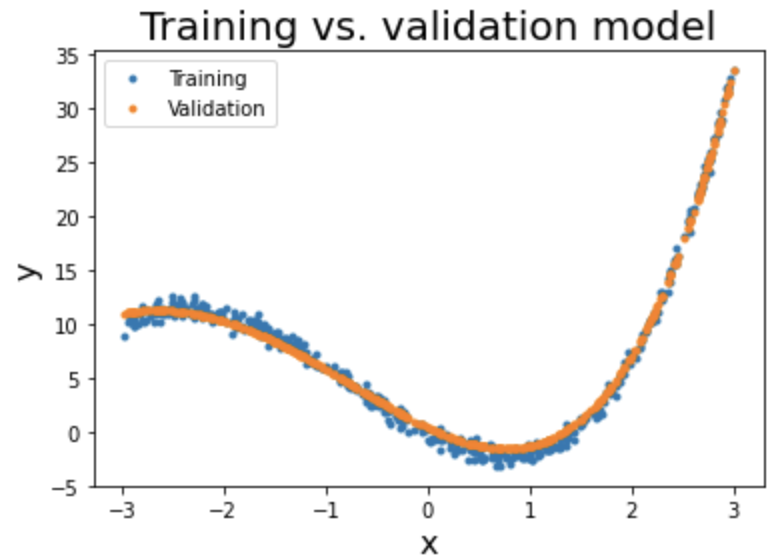
\includegraphics[scale = 0.7]{Question7_Graph.png}
\caption{\label{fig:fig}Graph for Question 1.7, validation and training model}
\end{figure}

\newpage

\subsection{Question 1.8}

The validation and training losses from the above trained model are depicted as follows:

\begin{figure}[!htb]
\centering
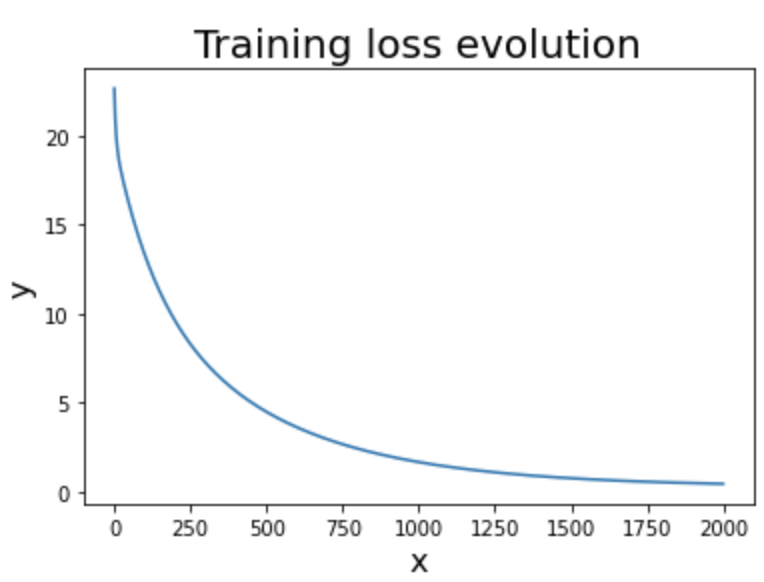
\includegraphics[scale = 0.8]{Question8_Graph1.png}
\caption{\label{fig:fig}Graph for Question 1.8, training losses}
\end{figure}

And respectively:

\begin{figure}[!htb]
\centering
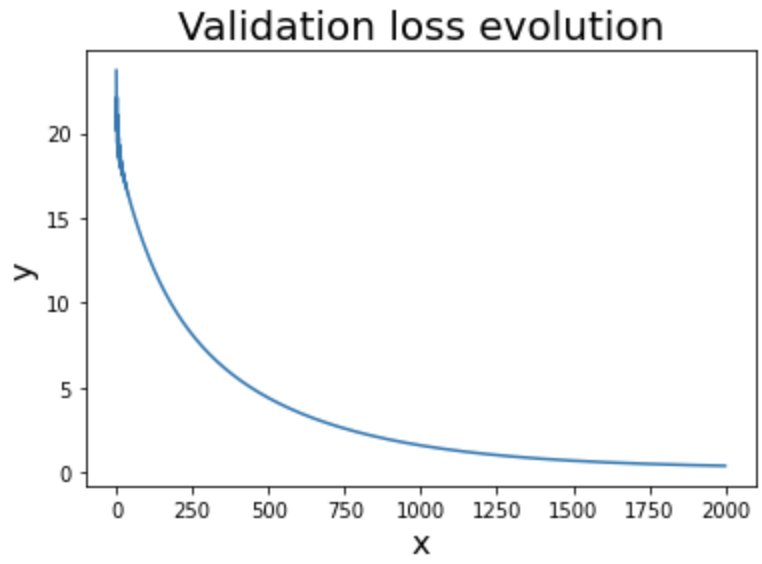
\includegraphics[scale = 0.8]{Question8_Graph2.png}
\caption{\label{fig:fig}Graph for Question 1.8, validation losses}
\end{figure}


\subsection{Question 1.9}

The evolution of w based on the results obtained in question 1.7 can be visualized as follows:

\begin{figure}[!htb]
\centering
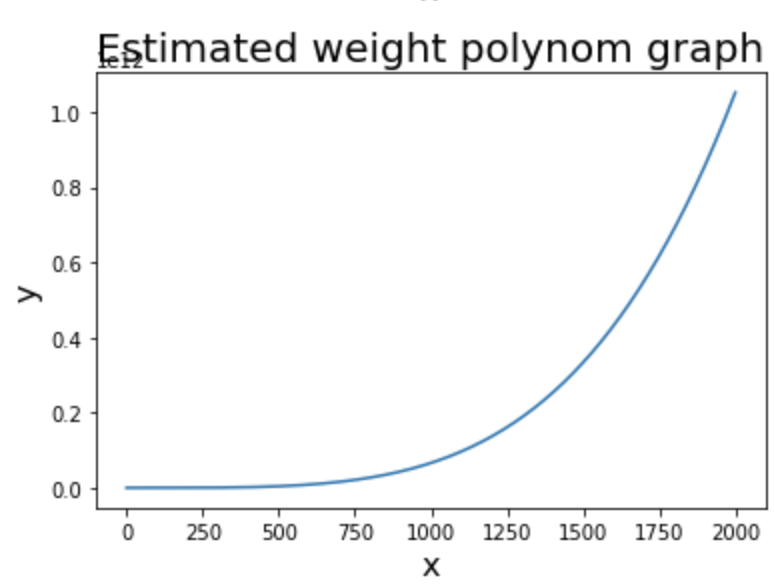
\includegraphics[scale = 0.8]{Question9_Graph.png}
\caption{\label{fig:fig}Graph for Question 1.9, polynomial defined by the estimate of w (obtained by question 1.7)}
\end{figure}


\subsection{Question 1.10}

The validation loss does not decrease as fast as compared to when more data sets are available. Furthermore, the training loss evolution converges, but also slower.
!!!!!! READ MORE INTO IT

\begin{figure}[!htb]
\centering
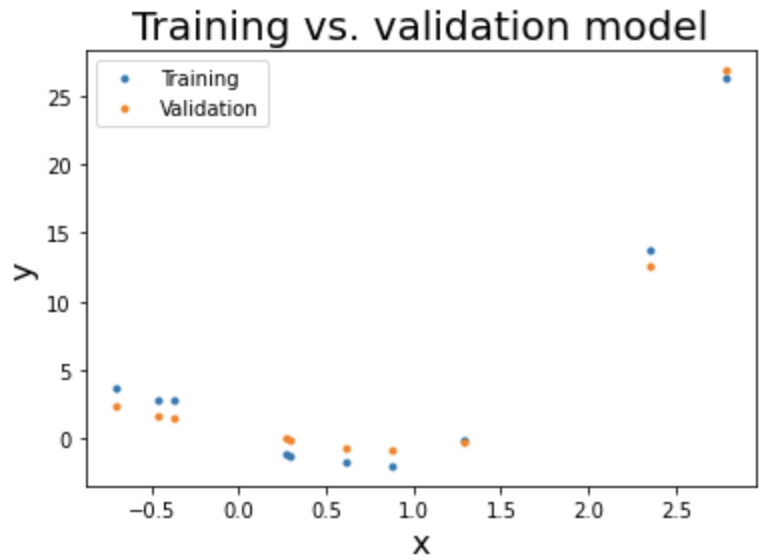
\includegraphics[scale = 0.8]{Question10_Graph1.png}
\caption{\label{fig:fig}Graph for Question 1.10, the visualization of training and validation set with reduced observations(10)}
\end{figure}


\begin{figure}[!htb]
\centering
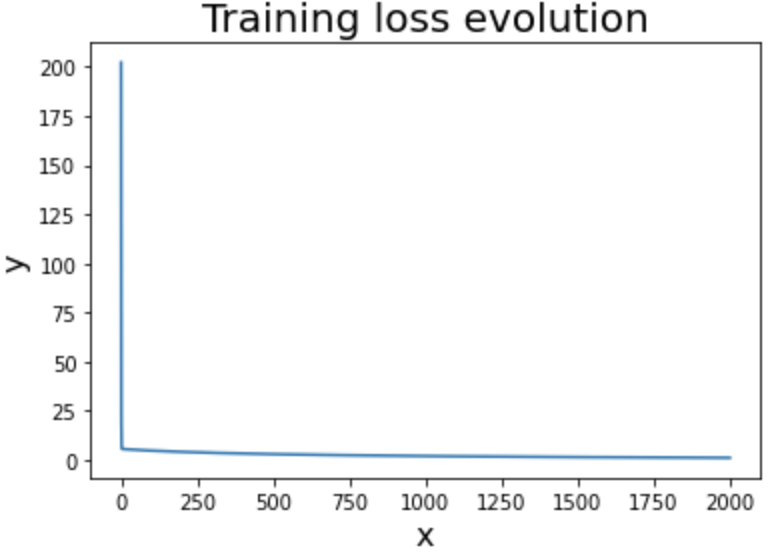
\includegraphics[scale = 0.8]{Question10_Graph2.png}
\caption{\label{fig:fig}Graph for Question 1.10, training losses with reduced observations (10)}
\end{figure}

\begin{figure}[!htb]
\centering
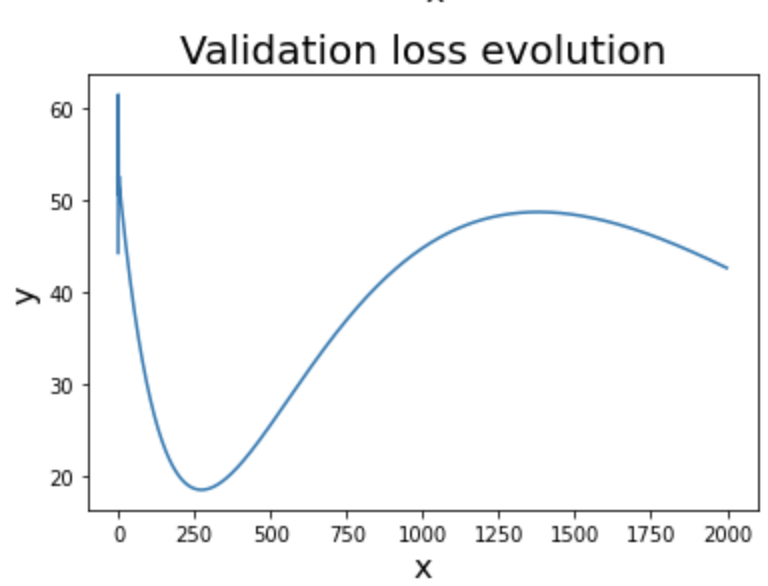
\includegraphics[scale = 0.8]{Question10_Graph3.png}
\caption{\label{fig:fig}Graph for Question 1.10, validation losses with reduced observations (10)}
\end{figure}

\newpage

\subsection{Question 1.11 - Bonus}

The following is the visualizaiton of the polynomial defined by the estimate of w obtained by question 1.7.

\begin{figure}[!htb]
\centering
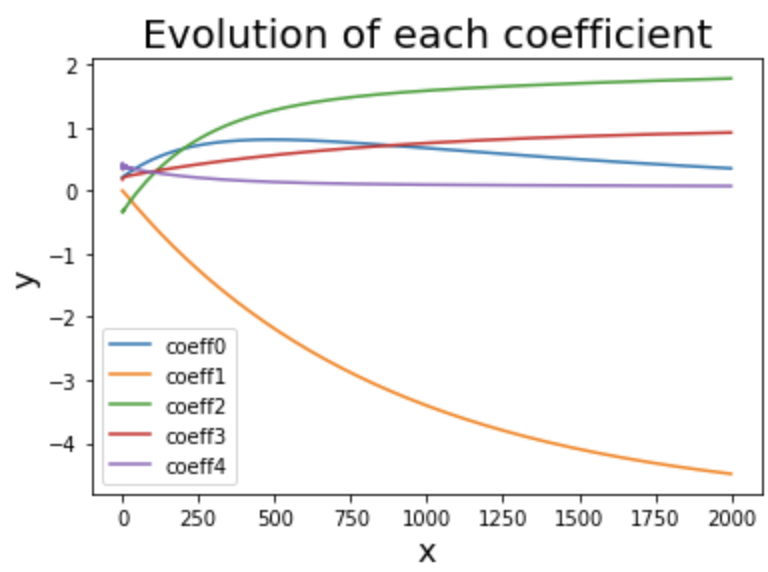
\includegraphics[scale = 0.8]{Question11_Graph.png}
\caption{\label{fig:fig}Graph for Question 1.11, visualization of the polynomial with obtained coefficient of Question 1.7}
\end{figure}

\newpage
\section{Question 2 [4/100 points]}

\subsection{Question 2.1}

\subsection{2.2}

\end{document}